% CVPR 2022 Paper Template
% based on the CVPR template provided by Ming-Ming Cheng (https://github.com/MCG-NKU/CVPR_Template)
% modified and extended by Stefan Roth (stefan.roth@NOSPAMtu-darmstadt.de)

\documentclass[10pt,twocolumn,letterpaper]{article}

%%%%%%%%% PAPER TYPE  - PLEASE UPDATE FOR FINAL VERSION %%%%%%%%%
%\usepackage[review]{cvpr}      % To produce the REVIEW version
%\usepackage{cvpr}              % To produce the CAMERA-READY version
\usepackage[pagenumbers]{cvpr} % To force page numbers, e.g. for an arXiv version

% Include other packages here, before hyperref.
\usepackage{graphicx}
\usepackage{amsmath}
\usepackage{amssymb}
\usepackage{booktabs}
\usepackage{float}
\usepackage{arydshln}
\usepackage{enumitem}


% It is strongly recommended to use hyperref, especially for the review version.
% hyperref with option pagebackref eases the reviewers' job.
% Please disable hyperref *only* if you encounter grave issues, e.g. with the
% file validation for the camera-ready version.
%
% If you comment hyperref and then uncomment it, you should delete
% ReviewTempalte.aux before re-running LaTeX.
% (Or just hit 'q' on the first LaTeX run, let it finish, and you
%  should be clear).
\usepackage[pagebackref,breaklinks,colorlinks]{hyperref}


% Support for easy cross-referencing
\usepackage[capitalize]{cleveref}
\crefname{section}{Sec.}{Secs.}
\Crefname{section}{Section}{Sections}
\Crefname{table}{Table}{Tables}
\crefname{table}{Tab.}{Tabs.}

\raggedbottom
\begin{document}

%%%%%%%%% TITLE - PLEASE UPDATE %%%%%%%%%
\title{DLP Lab5: Value-Based Reinforcement Learning}

\author{Yi-Hsiang Ho, 111550106
% For a paper whose authors are all at the same institution,
% omit the following lines up until the closing ``}''.
% Additional authors and addresses can be added with ``\and'',
% just like the second author.
% To save space, use either the email address or home page, not both
% \and
% Second Author\\
% Institution2\\
% First line of institution2 address\\
% {\tt\small secondauthor@i2.org}
}
\maketitle

%%%%%%%%% BODY TEXT %%%%%%%%%

\section{Introduction}
\label{sec:intro}

In this lab, I implemented and evaluated Value-Based Reinforcement Learning
algorithms, specifically Deep Q-Networks (DQN) and several of its enhancements.
The tasks involved solving two environments from the OpenAI Gymnasium: \textbf{
CartPole-v1} and \textbf{ALE/Pong-v5}.

The report is organized as follows: Section \ref{sec:impl} describes the
implementation details for Task 1 (Baseline DQN) and the subsequent enhancements
(Double DQN, Dueling DQN, PER, and Multi-step returns). Section \ref{sec:analysis}
provides a detailed analysis of the training performance, sample efficiency, and an
ablation study of the techniques used.

Key findings include:
\begin{itemize}[itemsep=-3pt]
  \item \verb|--epsilon-decay| affects the speed of convergence much.
  \item Enhancements like Double DQN and Multi-step returns significantly stabilize
    training and improve sample efficiency.
  \item Prioritized Experience Replay (PER) effectively focuses the agent's
    learning on more ``surprising'' transitions, leading to faster convergence.
  \item Dueling architecture helps the agent distinguish between state value and
    action advantage, which is particularly useful in Pong where many frames do not
    immediate impact the outcome.
\end{itemize}

\section{Implementation Details}
\label{sec:impl}

\subsection{DQN and Bellman Error}

The basic DQN uses a neural network to approximate the Q-value function $Q(s, a)$.
The network is trained by minimizing the Mean Squared Error (MSE) between the
predicted Q-values and the temporal difference (TD) targets.

\textbf{Bellman Error}: In my implementation, the Bellman error (or TD error) is
calculated as:
\begin{equation}
\delta = \left( r + \gamma \max_{a'} Q_{\text{target}}(s', a') \right) - Q_{\text{online}}(s, a)
\end{equation}
which code in shown in \cref{fig:impl-bellman}.

\begin{figure}[H]
  \centering
  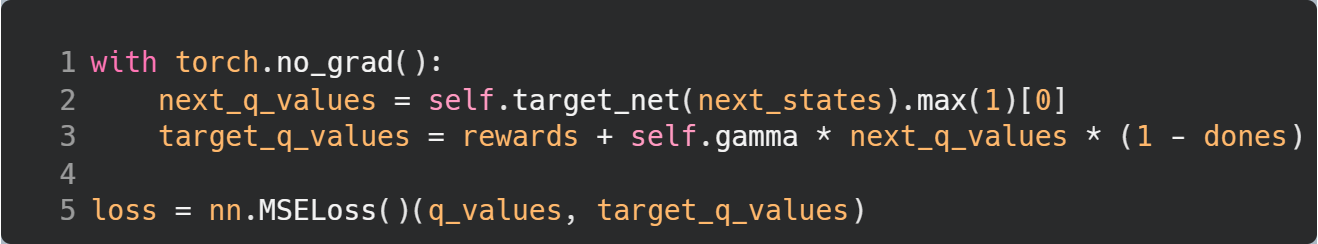
\includegraphics[width=\linewidth]{assets/impl-bellman.png}
  \caption{\textbf{Bellman Error Implementation}.}
  \label{fig:impl-bellman}
\end{figure}

During training, the loss $\mathcal{L} = \mathbb{E}[\delta^2]$ is minimized. In
Task 3, the TD error is detached from the computation graph and its absolute
value $|\delta|$ is used as the priority for the memory buffer. And also the
Huber loss is used instead of MSE loss.

\subsection{Double DQN (DDQN)}

Instead of using the target network for both selecting and evaluating the best
action, I used the online network to select the action and the target network
to evaluate it:
\begin{equation}
y_t^{\text{DDQN}} = r_t + \gamma Q_{\text{target}}\left( s_{t+1}, \arg\max_a Q_{\text{online}}(s_{t+1}, a) \right)
\end{equation}
In my code (\cref{fig:impl-ddqn}), this is implemented by passing the online
network's \verb|argmax| action to the target network's evaluation.

\begin{figure}[H]
  \centering
  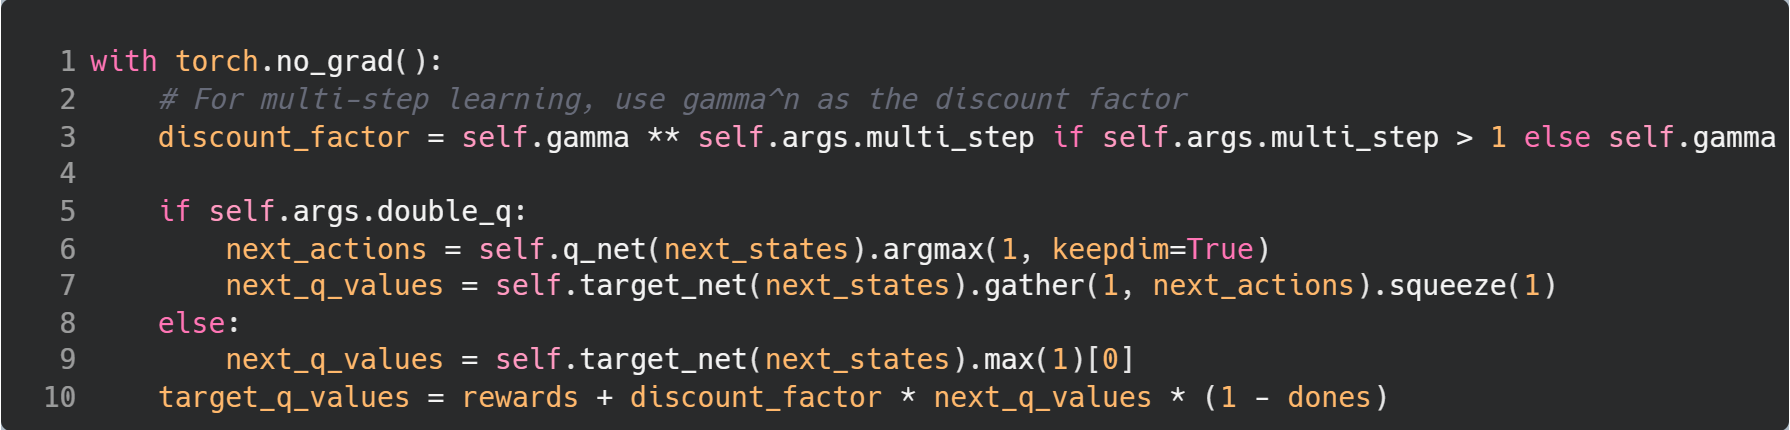
\includegraphics[width=\linewidth]{assets/impl-ddqn.png}
  \caption{\textbf{Double DQN Implementation}.}
  \label{fig:impl-ddqn}
\end{figure}

\subsection{Prioritized Experience Replay (PER)}

Instead of sampling transitions uniformly from the replay buffer, PER samples
transitions with higher TD errors more frequently, as they represent experiences
from which the agent can learn the most.

I implemented a SumTree data structure to allow $O(\log N)$ priority updates
and sampling. The probability of sampling transition $i$ is
$P(i) = \frac{p_i^\alpha}{\sum_k p_k^\alpha}$,
where $p_i = |\delta_i| + \epsilon$. To correct for the bias introduced by
non-uniform sampling, I used Importance
Sampling (IS) weights:
\begin{equation}
w_i = \left( \frac{1}{N \cdot P(i)} \right)^\beta
\end{equation}
where $\beta$ is annealed from 0.4 to 1.0 during training. This weight will
then be normalized by $\max(w_i)$ so it will be in range $[0, 1]$. In my implementation,
the $w_i$ is multiplied to the loss when calculating the TD error.

The code is in \verb|PrioritizedReplayBuffer| class in \verb|dqn_task3.py|.

\subsection{Multi-step Returns}

Multi-step returns (n-step) improve the bias-variance tradeoff in RL by
bootstrapping after $n$ steps instead of just one.

I maintained a small buffer (\verb|deque| of size $n=3$) to accumulate rewards
over $n$ steps:
\begin{equation}
G_t^{(n)} = \sum_{k=0}^{n-1} \gamma^k r_{t+k} + \gamma^n \max_a Q_{\text{target}}(s_{t+n}, a)
\end{equation}
and store this transition as a single element in replay buffer. That's also why
\cref{fig:impl-ddqn} need to compute $\gamma^k$ first, since the samples from
memory have already been $n$-step returns. The implementation is in
\cref{fig:impl-multi_step}.

\begin{figure}[H]
  \centering
  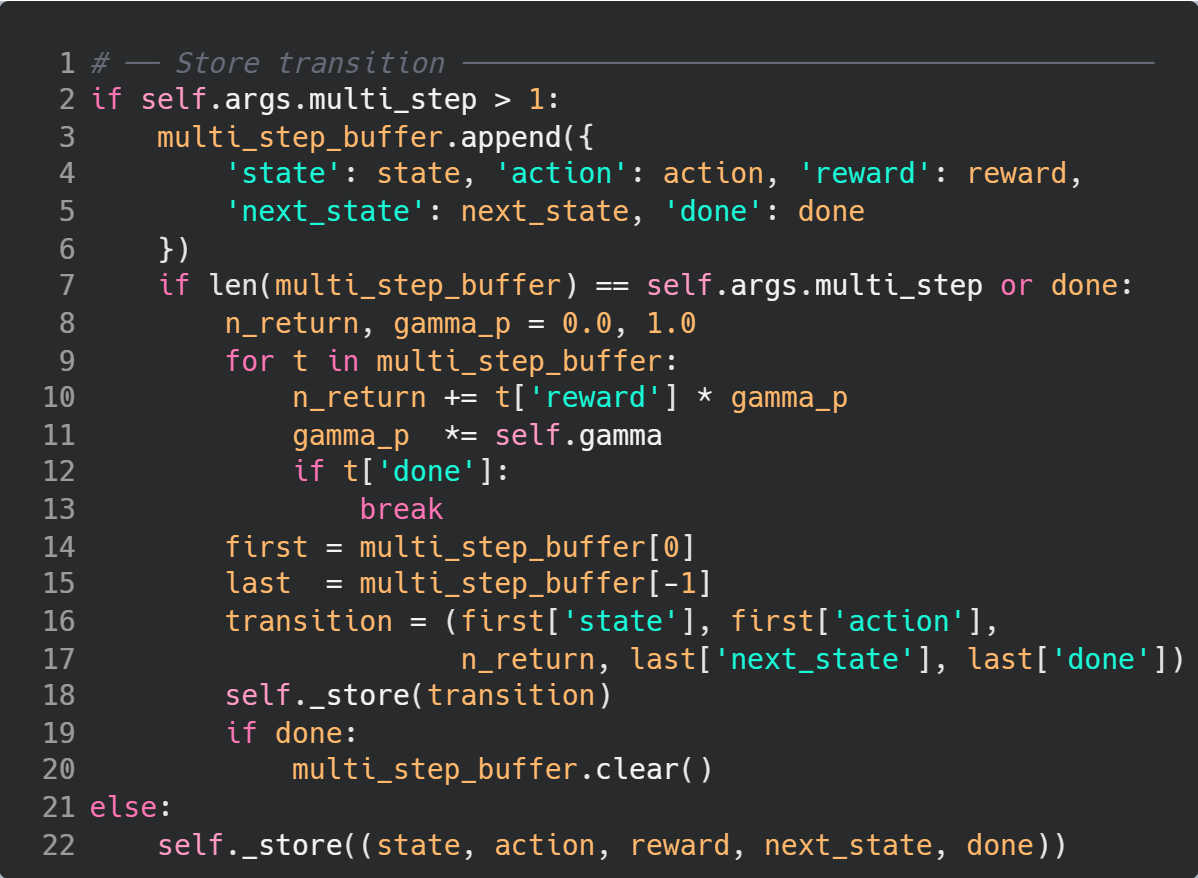
\includegraphics[width=\linewidth]{assets/impl-multi_step.png}
  \caption{\textbf{Multi-step Returns Implementation}.}
  \label{fig:impl-multi_step}
\end{figure}

\subsection{Tracking Performance with WandB}

I used \textbf{Weights \& Biases (WandB)} to track the model's performance in real-time. I logged:
\begin{itemize}[itemsep=-3pt]
  \item \verb|Total Reward|: Sum of rewards obtained in a single training episode.
  \item \verb|Eval Reward|: Average reward over multiple evaluation episodes (without exploration).
  \item \verb|Env Step Count|: Since I forgot setting x-axis for logging, All the following plots are redrawn with this as x-axis.
  \item \verb|Episode|, \verb|Epsilon|, and \verb|Update Count| for debugging.
\end{itemize}

\subsection{Addition: Dueling Network}

The \textbf{Dueling DQN} architecture improves upon the standard DQN by
separating the estimation of state-value $V(s)$ and action-advantage $A(s, a)$.
This is particularly useful in environments like Pong, where many states are
"neutral" (e.g., the ball is far from the paddle), and the specific action taken
has little impact on the immediate value of the state.

The Q-value is reconstructed as:
\begin{equation}
Q(s, a) = V(s) + \left( A(s, a) - \frac{1}{|\mathcal{A}|} \sum_{a' \in \mathcal{A}} A(s, a') \right)
\end{equation}
By subtracting the mean of the advantages, we ensure that the $Q$ values are
centered around $V(s)$, improving training stability. I implemented this by splitting
the final layers of the CNN into two separate streams: one for $V(s)$ (output
dimension 1) and one for $A(s, a)$ (output dimension $|A|$). The code snippet is in
\cref{fig:impl-duel}.

\begin{figure}[H]
  \centering
  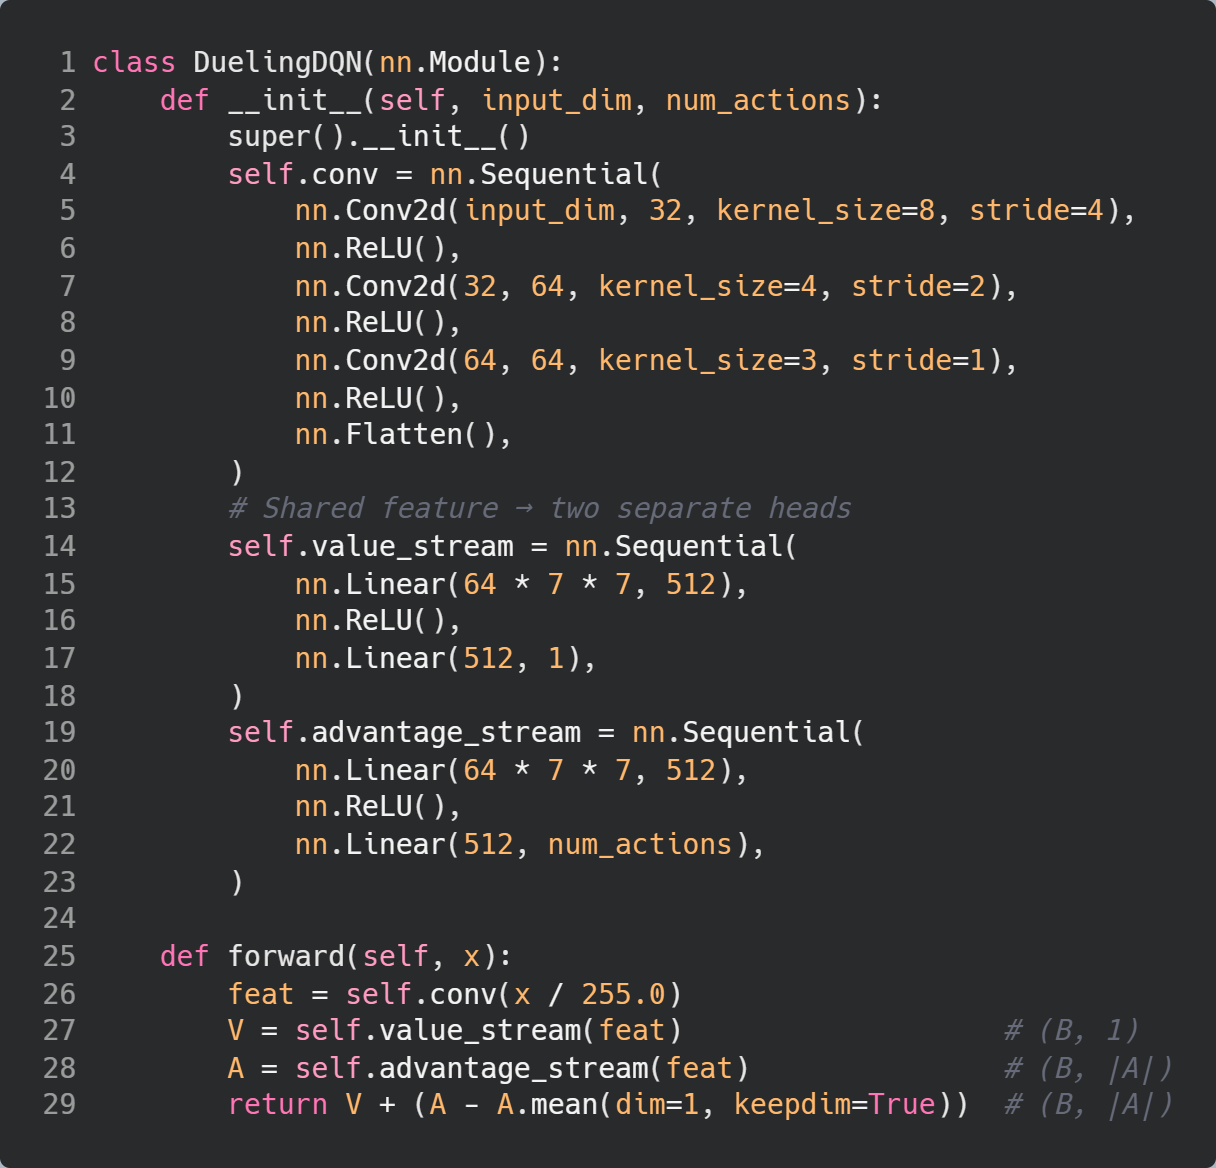
\includegraphics[width=\linewidth]{assets/impl-duel.png}
  \caption{\textbf{Dueling Network Architecture}.}
  \label{fig:impl-duel}
\end{figure}

\subsection{Addition: Action Reduction}

In the \verb|Pong-v5| environment, the default action space contains 6
actions: \verb|NOOP|, \verb|FIRE|, \verb|RIGHT|, \verb|LEFT|, \verb|RIGHTFIRE|,
and \verb|LEFTFIRE|. However, in Pong, movement is only vertical, and many of
these actions are redundant (e.g., \verb|FIRE| is often just a \verb|NOOP|).

I implemented a custom \verb|gym.ActionWrapper| in \cref{fig:impl-act_reduce}
to reduce the action space from 6
to 3:
\begin{itemize}[itemsep=-3pt]
  \item 0: \verb|NOOP|
  \item 1: \verb|UP| (mapped from \verb|RIGHT|)
  \item 2: \verb|DOWN| (mapped from \verb|LEFT|)
\end{itemize}
This reduction significantly accelerates training because the $\epsilon$-greedy
exploration policy is twice as likely to pick a meaningful movement action, and
the network does not waste capacity learning identical Q-values for redundant
outputs.

\begin{figure}[H]
  \centering
  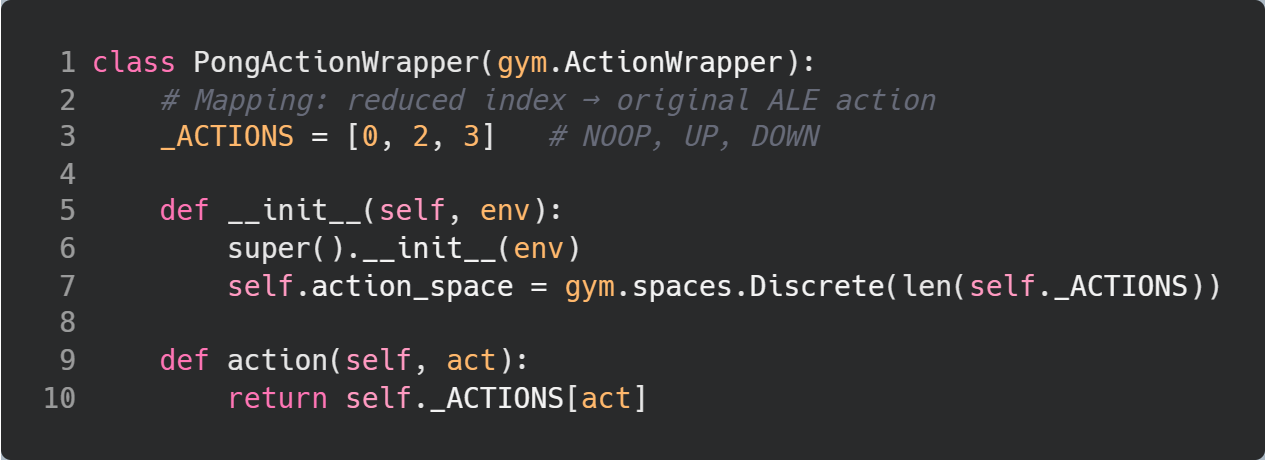
\includegraphics[width=\linewidth]{assets/impl-act_reduce.png}
  \caption{\textbf{Action Reduction Implementation}.}
  \label{fig:impl-act_reduce}
\end{figure}

\section{Analysis and Discussion}
\label{sec:analysis}

\subsection{Training Curves}

\textbf{Task 1 (CartPole)}: As shown in \cref{fig:task1}, the basic DQN agent
solves CartPole-v1 very quickly, reaching the maximum score of 500 within
approximately 20k-30k environment steps. The performance is highly stable once
converged. And the evaluation screenshot is in \cref{fig:task1-eval}. It successfully
reach maximum score 500 in 20 random seed tests.

\begin{figure}[H]
  \centering
  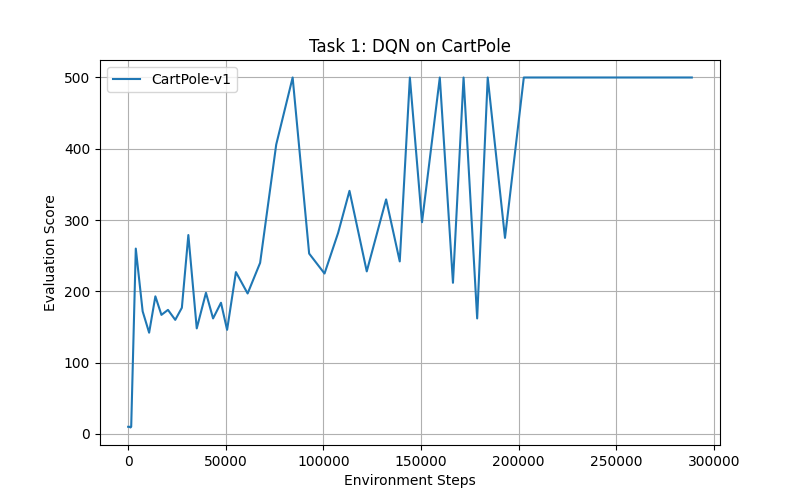
\includegraphics[width=\linewidth]{assets/task1_curve.png}
  \caption{\textbf{Training curve for CartPole-v1 (Task 1)}.}
  \label{fig:task1}
\end{figure}

\begin{figure}[H]
  \centering
  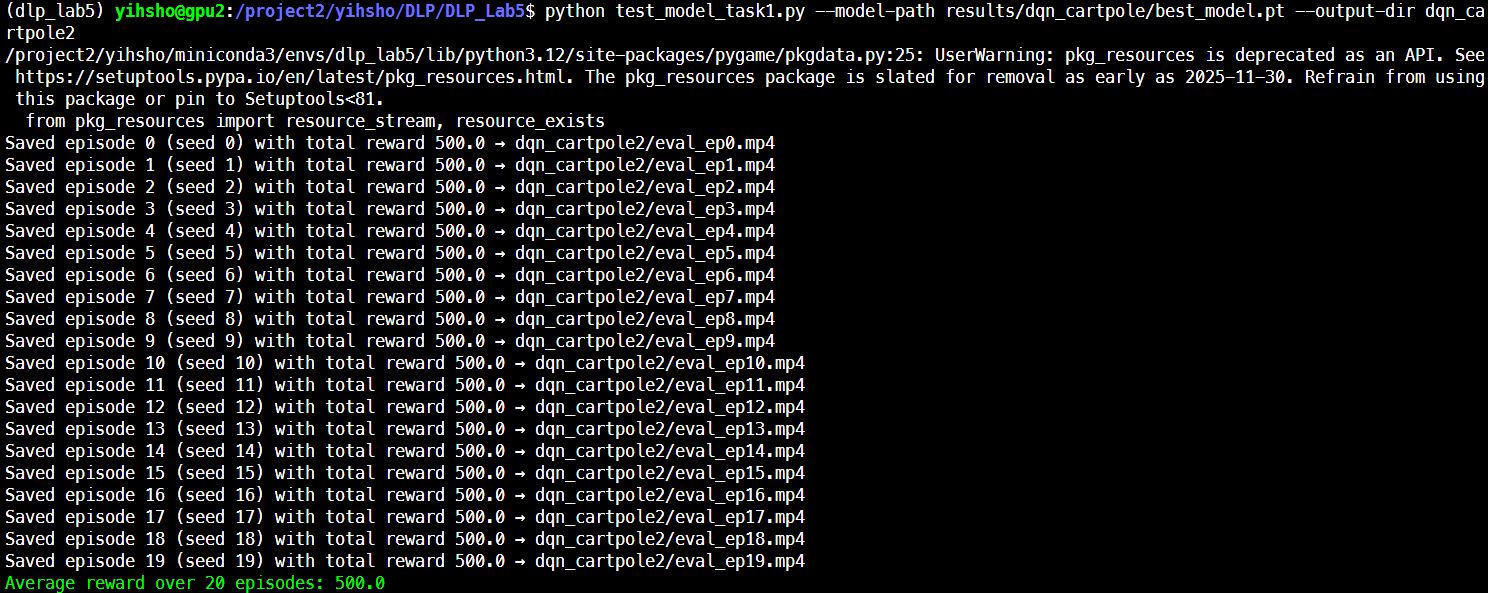
\includegraphics[width=\linewidth]{assets/task1_eval.png}
  \caption{\textbf{Evaluation for CartPole-v1 (Task 1)}. Test with 20 random seed.}
  \label{fig:task1-eval}
\end{figure}

\textbf{Task 2 (Pong Baseline)}: In \cref{fig:task2}, the baseline DQN
(without enhancements) eventually solves Pong, but it requires
significantly much more environment steps (over 4M) to steadily achieve
score above 19. Moreover, it also exhibits higher variance during training,
as shown in figure, the evaluation score still drops a lot even when it
achieves high score, indicating the training is unstable. In my experiment,
the best score is 19.3 at around 5M steps. The screenshot is in
\cref{fig:task2-eval}

\begin{figure}[H]
  \centering
  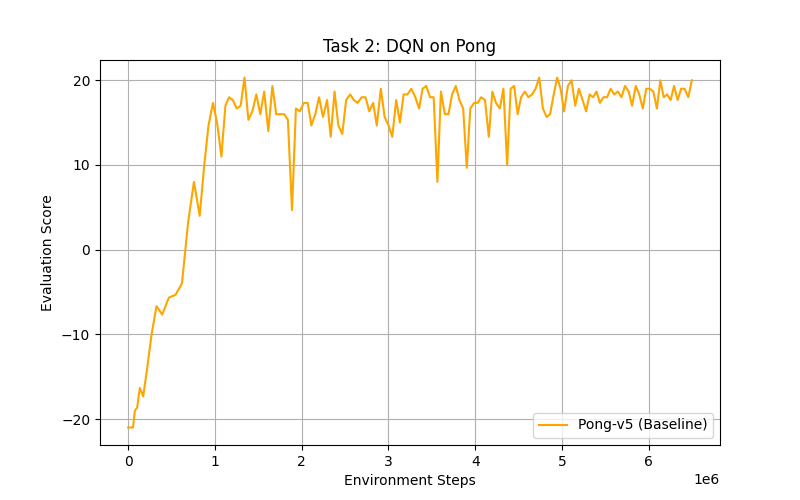
\includegraphics[width=\linewidth]{assets/task2_curve.png}
  \caption{\textbf{Training curve for Pong-v5 (Task 2, Baseline DQN).}}
  \label{fig:task2}
\end{figure}

\begin{figure}[H]
  \centering
  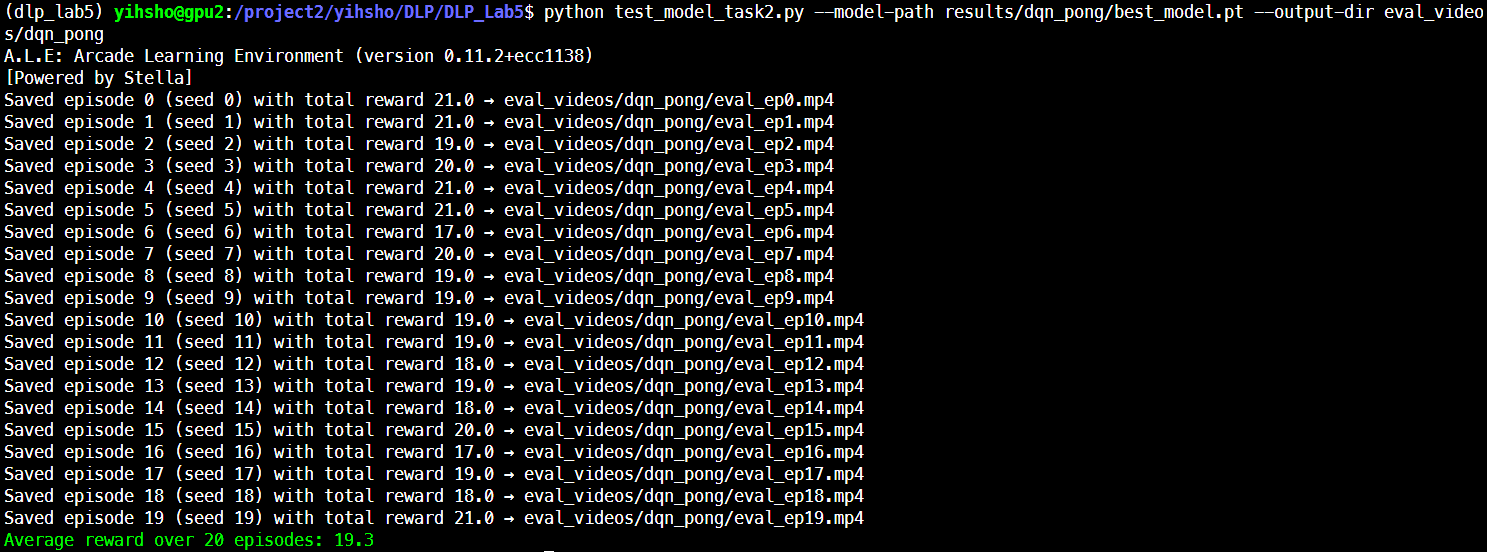
\includegraphics[width=\linewidth]{assets/task2_eval.png}
  \caption{\textbf{Evaluation for Pong-v5 (Task 2, Baseline DQN).} Test with 20 random seed.}
  \label{fig:task2-eval}
\end{figure}

\textbf{Task 3 (Enhanced Pong)}: The agent with four enhancements
(DDQN, Dueling, PER, Multi-step) and replacing loss function from MSE to
Huber loss reaches a high score (above 19) much faster and more reliably
than the baseline, as shown in \cref{fig:task3} and \cref{tab:task3-eval}.
Since the checkpoints are saved in the end of each episode, the environment
step in the figure is not exactly match the 600k, 1M, etc. But generally, it
is closed enough that will not affect the analysis. (The true steps are listed
in the caption of \cref{fig:task3-eval}).

\begin{table}[H]
  \centering
  \setlength{\tabcolsep}{5pt}
  \begin{tabular}{@{}lccccc@{}}
    \toprule
    \textbf{Method}   & \textbf{600k} & \textbf{1M}   & \textbf{1.5M} & \textbf{2M}   & \textbf{2.5M} \\
    \midrule
    Baseline DQN     & 0.2 & 16.45 & 16.1 & 16.8 & 16.45 \\
    Enhanced         & 10.8 & 18.1 & 18.95 & \textbf{19.45} & \textbf{19.95} \\
    \bottomrule
  \end{tabular}
  \caption{\textbf{Evaluation result in different steps}. It is tested
    with 20 random seed for each step. The score above 19 is marked in bold.}
  \label{tab:task3-eval}
\end{table}

\begin{figure}[H]
  \centering
  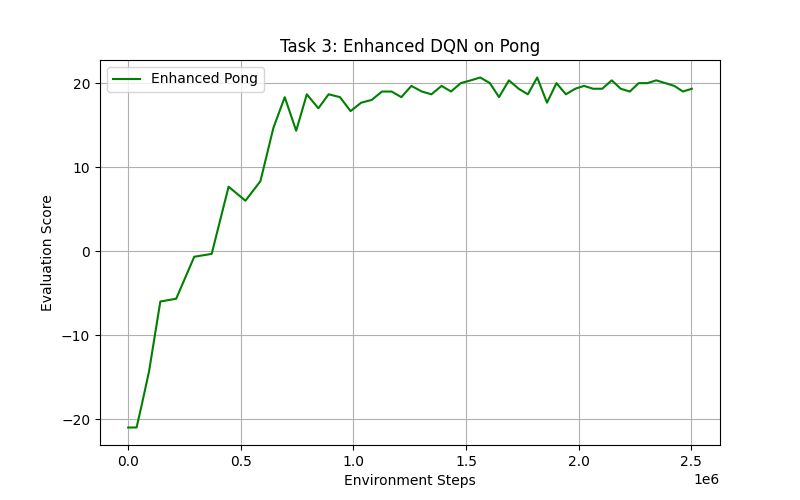
\includegraphics[width=\linewidth]{assets/task3_curve.png}
  \caption{\textbf{Training curve for Enhanced Pong (Task 3).}}
  \label{fig:task3}
\end{figure}

\begin{figure}[H]
  \centering
  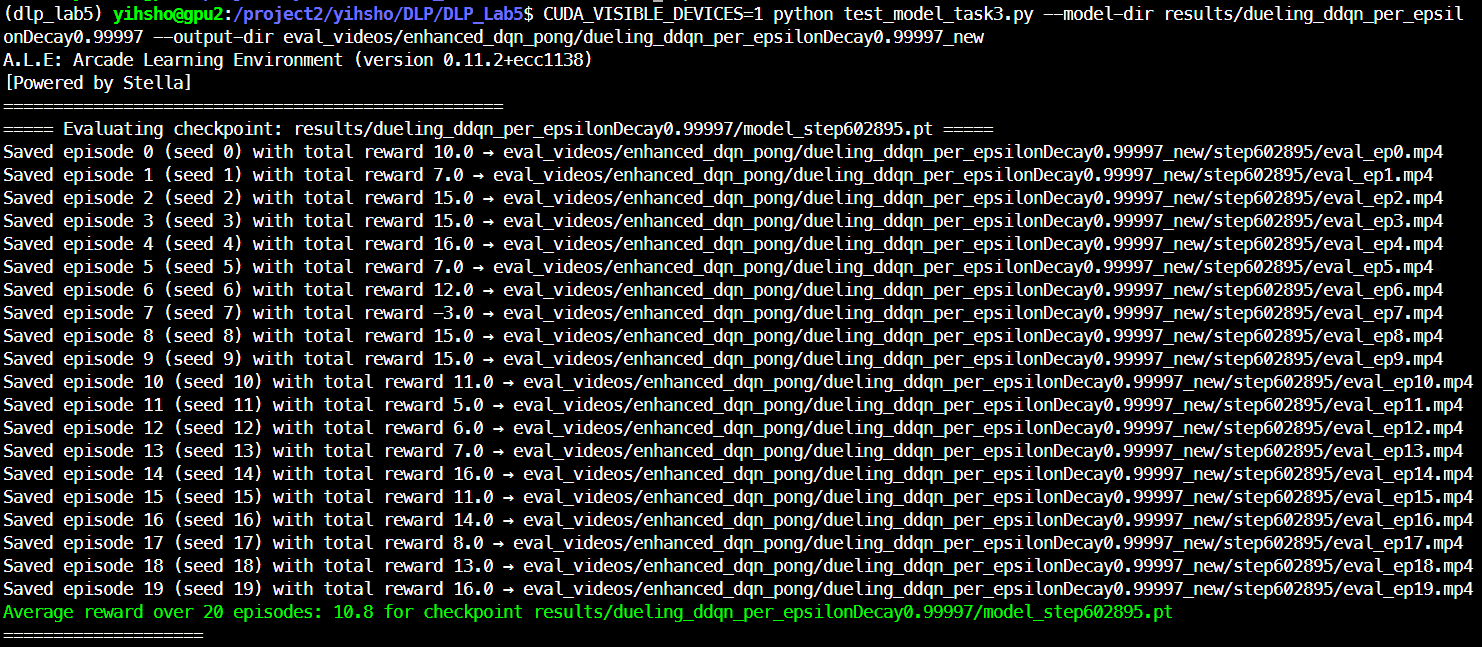
\includegraphics[width=\linewidth]{assets/task3_eval_step600k.png}
  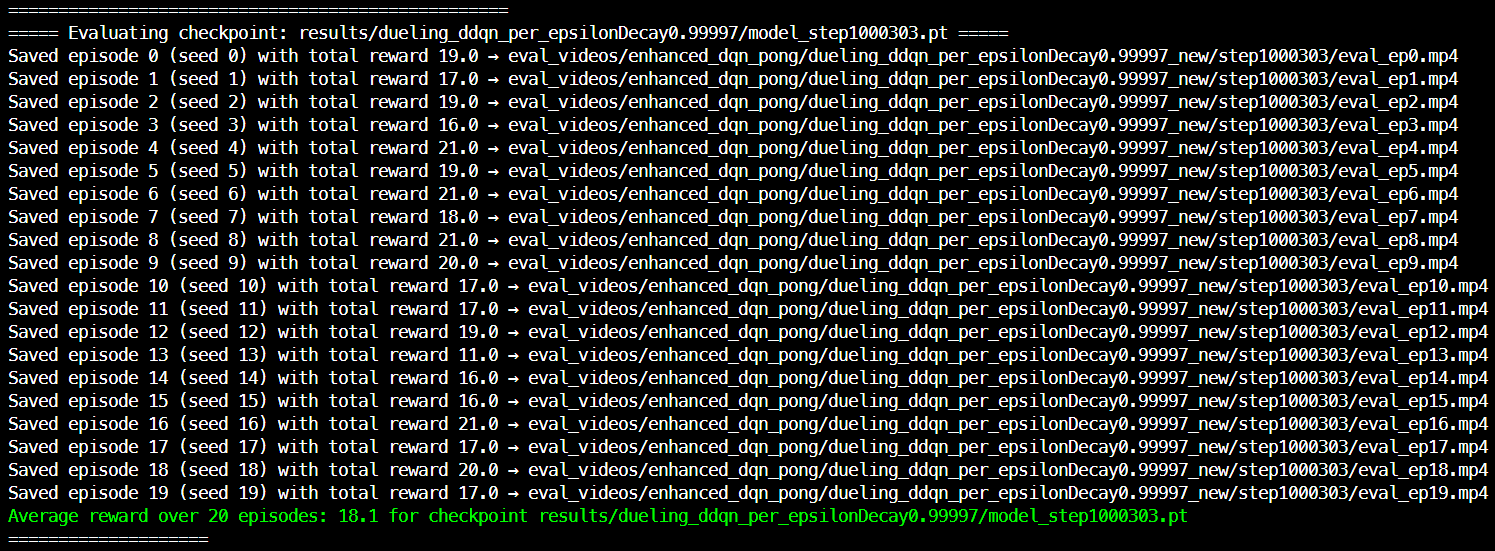
\includegraphics[width=\linewidth]{assets/task3_eval_step1M.png}
  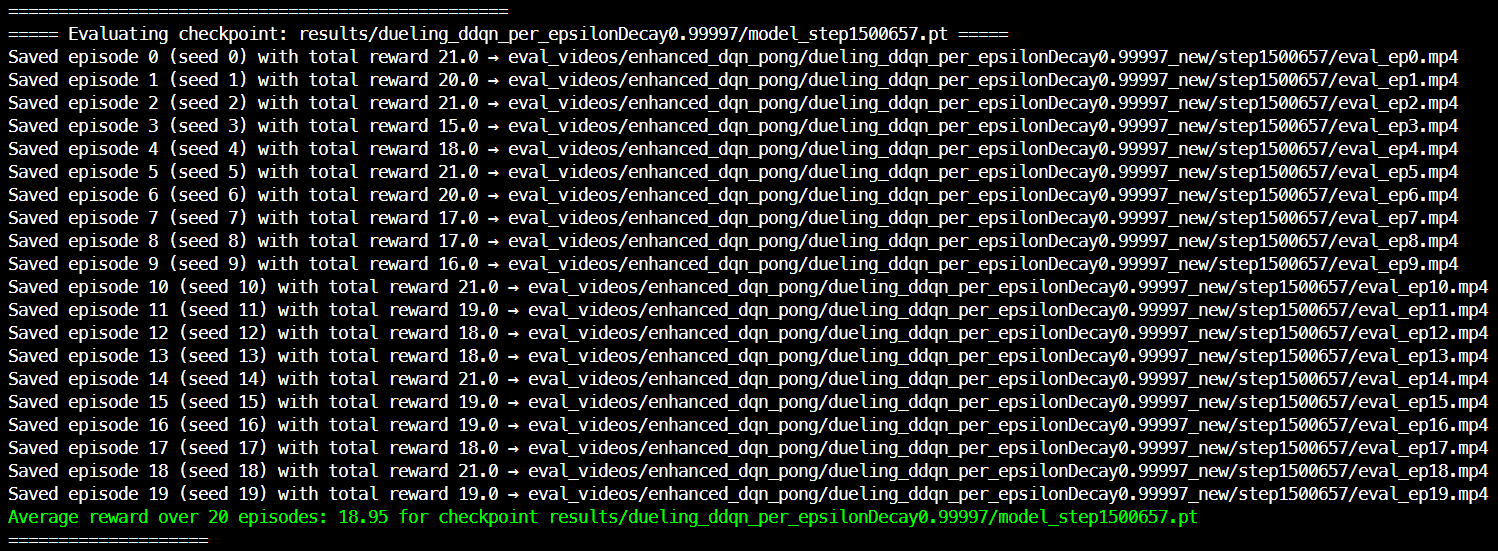
\includegraphics[width=\linewidth]{assets/task3_eval_step1.5M.png}
  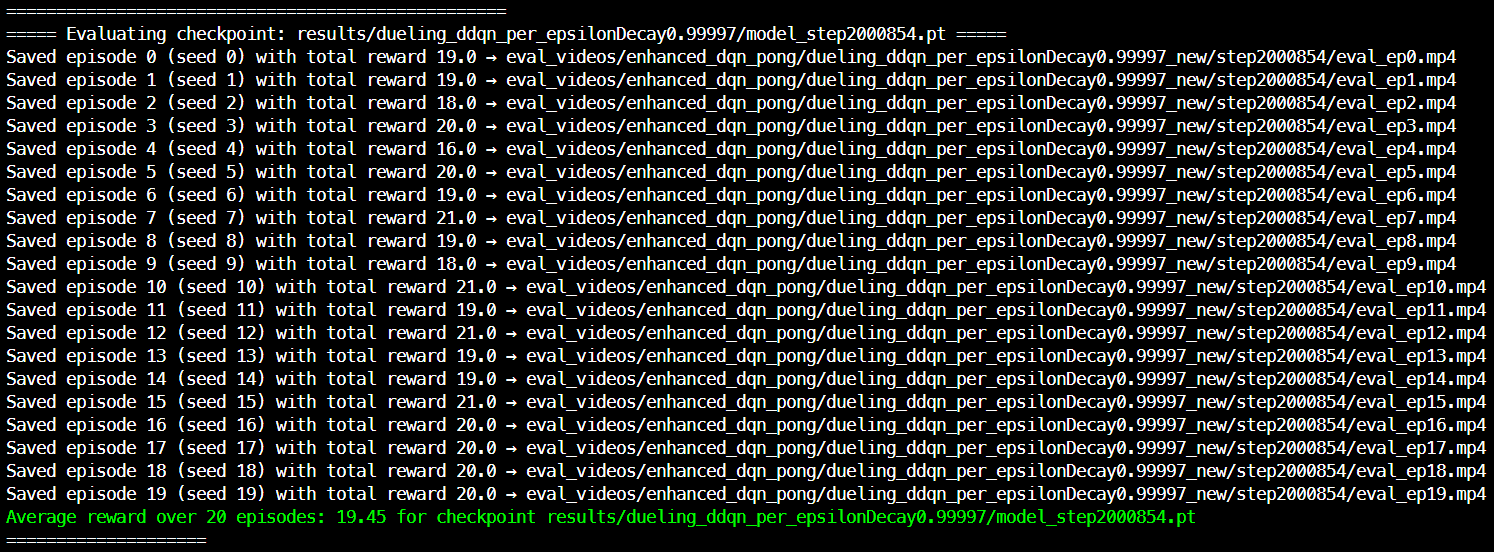
\includegraphics[width=\linewidth]{assets/task3_eval_step2M.png}
  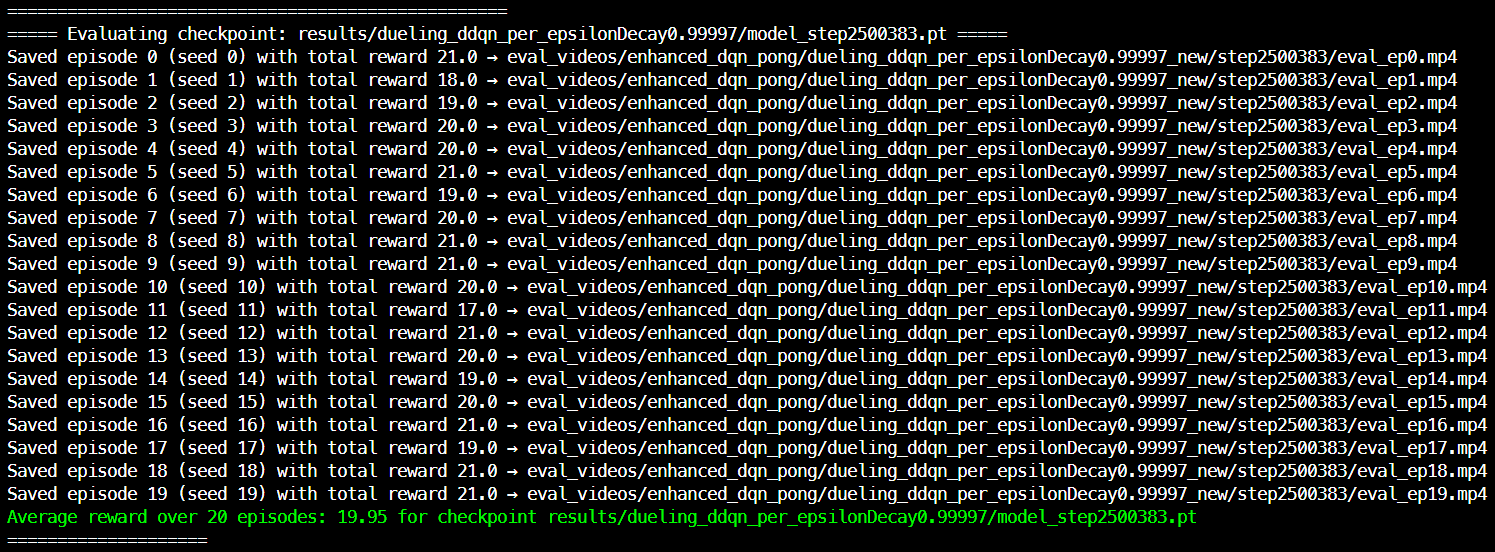
\includegraphics[width=\linewidth]{assets/task3_eval_step2.5M.png}
  \caption{\textbf{Evaluation for Enhanced Pong (Task 3).} Checkpoints
    were saved at 602895, 1000303, 1500657, 2000854, 2500383 environment steps.}
  \label{fig:task3-eval}
\end{figure}

\subsection{Sample Efficiency Analysis}

The DQN enhancements dramatically improved sample efficiency. As shown in
\cref{fig:sample-efficiency}, the baseline agent in Task 2 required approximately
800k steps to reach a positive evaluation score. In contrast, the enhanced
agent in Task 3 achieved a positive score around 350k to 400k steps,
effectively doubling the learning speed. Furthermore, the enhanced agent reached
a stable winning plateau (19 or higher) at 1.5M steps, while the baseline
agent took nearly 4M steps to reach a stable plateau.

This significant improvement is primarily due to:
\begin{enumerate}[itemsep=-3pt]
  \item \textbf{Multi-step returns}: Propagating rewards backward over 3 steps
  instead of 1, allowing for faster credit assignment.
  \item \textbf{Prioritized Experience Replay (PER)}: Ensuring that the agent
  revisits transitions with high TD-errors, focusing the learning on the most
  informative samples.
  \item \textbf{Dueling Architecture}: Better separating the state-value
  estimation from action-specific advantages, which is particularly useful in
  Pong where many states have similar values regardless of the move.
\end{enumerate}

\begin{figure}[H]
  \centering
  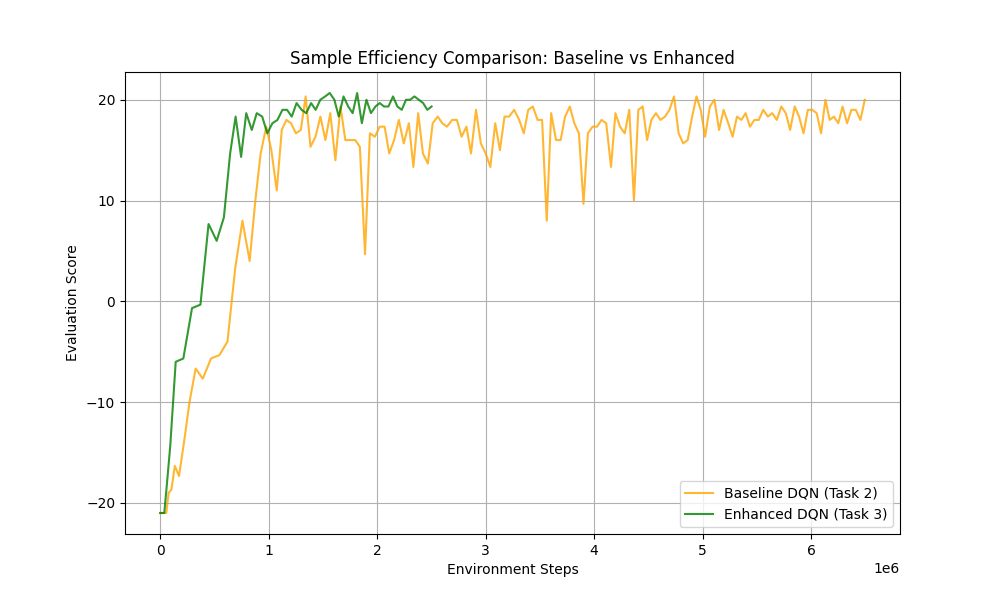
\includegraphics[width=\linewidth]{assets/sample_efficiency.png}
  \caption{Sample efficiency comparison between Baseline DQN (Task 2) and Enhanced DQN (Task 3).}
  \label{fig:sample-efficiency}
\end{figure}

\subsection{Ablation Study}

\begin{table}[H]
  \centering
  \setlength{\tabcolsep}{5pt}
  \begin{tabular}{@{}lccccc@{}}
    \toprule
    \textbf{Method}   & \textbf{600k} & \textbf{1M}   & \textbf{1.5M} & \textbf{2M}   & \textbf{2.5M} \\
    \midrule
    Baseline DQN     & 0.2 & 16.45 & 16.1 & 16.8 & 16.45 \\
    \addlinespace[0.5ex]
    \hdashline
    \addlinespace[0.5ex]
    Enhanced (All)   & 5.25 & 14.95 & 18.2 & \textbf{19.4} & 18.85 \\
    Enhanced 2 (All) & 10.33 & 16.67 & 17.33 & \textbf{19} & 18 \\
    w/o DDQN         & 1.67 & 7 & 5.67 & 15 & 17.33 \\
    w/o Dueling      & 18.33 & 16.67 & 18.33 & 17 & \textbf{19} \\
    w/o PER          & 4.33 & 7.67 & 12 & 16.33 & 13 \\
    w/o Multi-step   & 9.67 & 14.33 & 18.33 & 17.33 & 18.67 \\
    w/o Act-Reduce   & 6.33 & 16.67 & 16.33 & 17.33 & 18 \\
    w/o Act-Reduce 2 & 10.8 & 18.1 & 18.95 & \textbf{19.45} & \textbf{19.95} \\
    \bottomrule
  \end{tabular}
  \caption{\textbf{Comparison of different methods at specific training steps}. 
    The score above 19 is marked in bold.}
  \label{tab:ablation}
\end{table}

\begin{figure}[H]
  \centering
  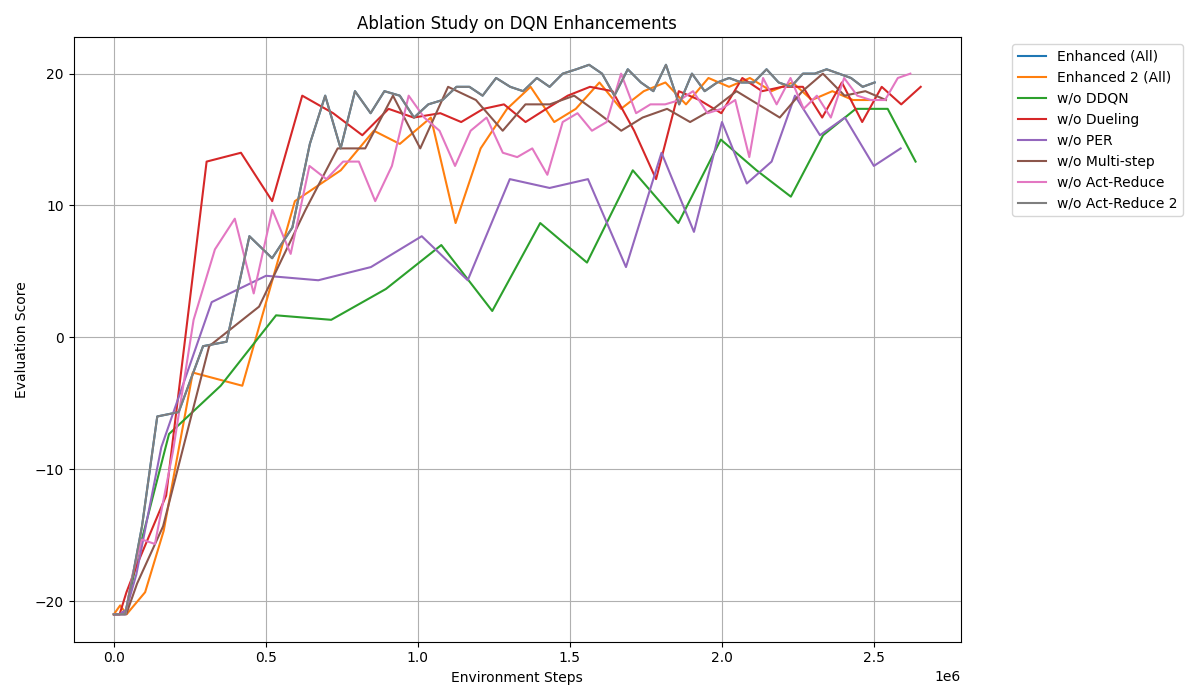
\includegraphics[width=\linewidth]{assets/ablation_study.png}
  \caption{Ablation study of DQN enhancements on Pong.}
  \label{fig:ablation}
\end{figure}

I performed an ablation study by removing each technique individually from the
Task 3 configuration. The results in \cref{fig:ablation} and \cref{tab:ablation}
show:
\begin{itemize}[itemsep=0pt]
  \item \textbf{w/o PER}: Most severe degradation, peaking at only 13.0. This confirms PER's critical role in prioritizing informative samples in sparse reward environments.
  \item \textbf{w/o Double DQN}: Significantly slowed early learning and limited the final score to 17.33, highlighting its importance in mitigating overestimation bias.
  \item \textbf{w/o Dueling}: Fastest early-stage learner (18.33 at 600k steps) but reached a similar final plateau (~19.0) as the enhanced versions.
  \item \textbf{w/o Multi-step}: Showed a slower start but eventually reached 18.67, indicating its primary benefit is accelerating early-stage credit assignment.
  \item \textbf{High Variance}: Configurations like \textit{w/o Act-Reduce 2} reached the highest final score (19.95), suggesting that training outcome is highly sensitive to initialization and exploration noise.
\end{itemize}

\section{Conclusion}

In this lab, I implemented and evaluated a series of DQN enhancements to solve the Pong-v5 environment. The combination of Double DQN, Dueling DQN, PER, and Multi-step returns significantly outperformed the baseline, achieving a 2x improvement in sample efficiency and much higher final scores.

Through the ablation study, I identified Prioritized Experience Replay (PER) and Double DQN as the most critical enhancements for reaching high performance and stability. The experiment also revealed substantial variance in training outcomes, where factor like random initialization sometimes allowed configurations without action space reduction to achieve the highest scores (+19.95). Overall, this lab demonstrated that while sophisticated algorithmic enhancements provide a robust foundation, careful hyperparameter tuning and an understanding of stochastic factors remain vital in deep reinforcement learning.

\section*{DISCLOSURE FOR AI TOOLS}

I used Copilot to help me write the code and report, and use Claude for ideas to
improve learning efficiency. However, I have checked and modified them to ensure
the correctness and quality.

% {\small
% \bibliographystyle{ieee_fullname}
% \bibliography{egbib}
% }

\end{document}